%===============================================================================
\section{CUDAHM motivation and design}
\label{sec:design}

%-------------------------------------------------------------------------------
\subsection{Motivating problem structures}
\label{sec:motiv}

Suppose we observe $N$ members of a large population, with the observed members indexed by $i=1$ to $N$.
Each object (member) has a property or properties $\psi_i$ (a vector in multiple-property cases); we are interested in estimating the collection of properties, $\{\psi_i\}$, or their distribution, but cannot measure every component of $\psi_i$ with high precision.
Instead, for each object, we have observed data, $D_i$, that provide information about $\psi_i$.
In the following, we sometimes use bold symbols to refer to quantities collectively, e.g., $\psivec \equiv \{\psi_i\}$, and $\Dvec \equiv \{D_i\}$.

We consider problems where the nature of the observations motivates models that specify a joint sampling distribution for the data, conditional on the member properties, that factors into a product of conditionally independent \emph{member sampling distributions},%
\footnote{For the sake of simplicity, we denote random variables and their values with the same symbol.
Also, $p(\bullet)$ will be used to denote a probability mass function or a probability density function, depending on the type of the argument.}
\begin{equation}
p(\Dvec \assm \psivec) = \prod_{i=1}^N p(D_i \assm \psi_i).
\label{data-joint-member}
\end{equation}
We model the member properties, $\psivec$, as IID draws from a \emph{population probability density function} (PPDF), $f(\psi_i;\theta)$, with uncertain parameters, $\theta$.
Goals of inference may include estimation of the PPDF (i.e., estimation of $\theta$), or estimation of the member properties, $\psivec$.

Fig.~\ref{fig:DAG-2Level} shows the DAG for this type of model, both explicitly and using plate notation.  Following standard conventions, open nodes indicate uncertain random variables that are targets of inference, and shaded nodes indicate observed quantities, i.e., random variables that are uncertain a priori, but that become known after observation, and thus may be conditioned on.
If we denote the prior PDF for the population distribution parameters by $\pi(\theta)$, this DAG indicates that the joint PDF for all random quantities in this model may be written,
\begin{align}
p(\theta, \{\psi_i\}, \{D_i\})
  &= \pi(\theta) \prod_{i=1}^N f(\psi_i;\theta)\, p(D_i \assm \psi_i)\\
  &\propto \pi(\theta) \prod_{i=1}^N f(\psi_i;\theta)\, \mlike_i(\psi_i),
\label{joint-2level}
\end{align}
where we have defined the \emph{member likelihood functions},
\[
\mlike_i(\psi_i) \propto p(D_i|\psi_i).
\label{mlike-def}
\]
Note that, as likelihood functions (vs.\ sampling distributions), these functions need only be specified up to proportionality.
In particular, any dependence on $D_i$ that does not influence the dependence on $\psi_i$ can be ignored.

\begin{figure}
\begin{center}
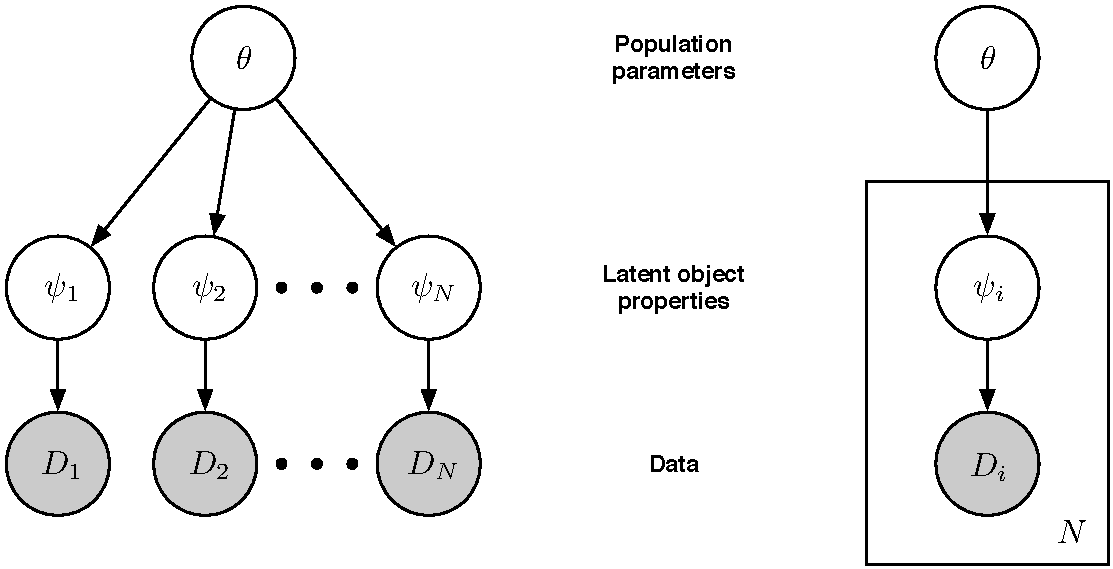
\includegraphics[width=.8\textwidth]{fig/DAG-2Level-Full+Plate}
\end{center}
\caption{Directed acyclic graph (DAG) for a 2-level hierarchical Bayesian model.
\emph{Left}:~DAG explicitly showing replicated conditionally independent subgraphs.
\emph{Right}:~DAG depicting replicated elements with a plate.}
\label{fig:DAG-2Level}
\end{figure}

The DAG describes a generative model for all of the random variables, including the data.
However, when the task is inference of parameters conditional on observed data (versus prediction of unobserved data), specifying member likelihood functions (rather than sampling distributions) can be a significant simplification.
In many astronomical applications, estimation of $\psi_i$ from $D_i$ is often a nontrivial inference problem in itself.
For example, when $\psi_i$ denotes the apparent brightness of a star and $D_i$ denotes image data, inference may involve fitting the complicated point spread function of an imaging instrument to Poisson distributed photon counts in dozens or hundreds of pixels (often marginalizing over an uncertain background or instrument calibration component).
The resulting likelihood function for $\psi_i$ (or marginal likelihood function, when there are nuisance parameters) will often be relatively easy to summarize as a function of $\psi_i$; e.g., it may be well approximated by a Gaussian or multivariate Gaussian function (perhaps after a transformation).
On the other hand, the sampling distribution for the data may be quite complicated and high-dimensional.
In many circumstances, it may not even be well-defined.
Weather or spacecraft conditions may affect the precision, accuracy, and even the quantity of data for a member observation; the repeated sampling distribution may be hard or even impossible to define objectively, while the likelihood function may be well-defined.
Most astronomical surveys produce member estimates with heteroscedastic uncertainties, in the sense of producing member likelihood functions with widths that vary from object to object.
It may be difficult or impossible to accurately describe the repeated sampling properties of the heteroscedastic uncertainties.
But for inference based on \emph{given} observations, only the actually available member likelihood functions matter.
Implementing inference in a manner that requires specifying only the member likelihood functions, rather than the sampling distributions, is a better fit to the nature of astronomical survey catalog data summaries than an implementation requiring unique specification of the lowest level sampling distributions.

A widely-used approach for posterior sampling in the context of two-level hierarchical models is the \textit{Metropolis-within-Gibbs} (MWG) algorithm, where the $\theta$ population parameters and the $\psi_i$ member properties are sampled in separate, alternating steps.
First, the member properties are sampled by holding the population parameters fixed, then the population parameters are sampled by holding the member properties fixed.
These steps may each be implemented with Metropolis or Metropolis-Hastings algorithms; their sequential combination amounts to Gibbs sampling on the joint space.
Explicitly, the steps are:
\begin{align}
\psi_i &\sim p(\psi_i \assm \theta, D_i), \quad\forall i\in 1:N;
\label{eq:psi_sampling} \\
\theta &\sim p(\theta \assm \psivec, M).
\label{eq:theta_sampling}
\end{align}
The departure point for CUDAHM is recognition that, since the $\psi_i$ properties are conditionally independent in \eqref{eq:psi_sampling}, they may be sampled in parallel, making this part of the MWG algorithm suitable for a massively parallel implementation using GPUs.
We describe such an implementation further below.

Since $\psi_i$ may be a vector, the $\psi_i$ node in the DAG may admit a factorization leading to further structure within the plate in Fig.~\ref{fig:DAG-2Level}.
Fig.~\ref{fig:DAGs} shows DAGs for several other single-plate modeling scenarios for which inference may be implemented using MWG with massively parallel sampling of member properties.

\begin{figure}
\begin{center}
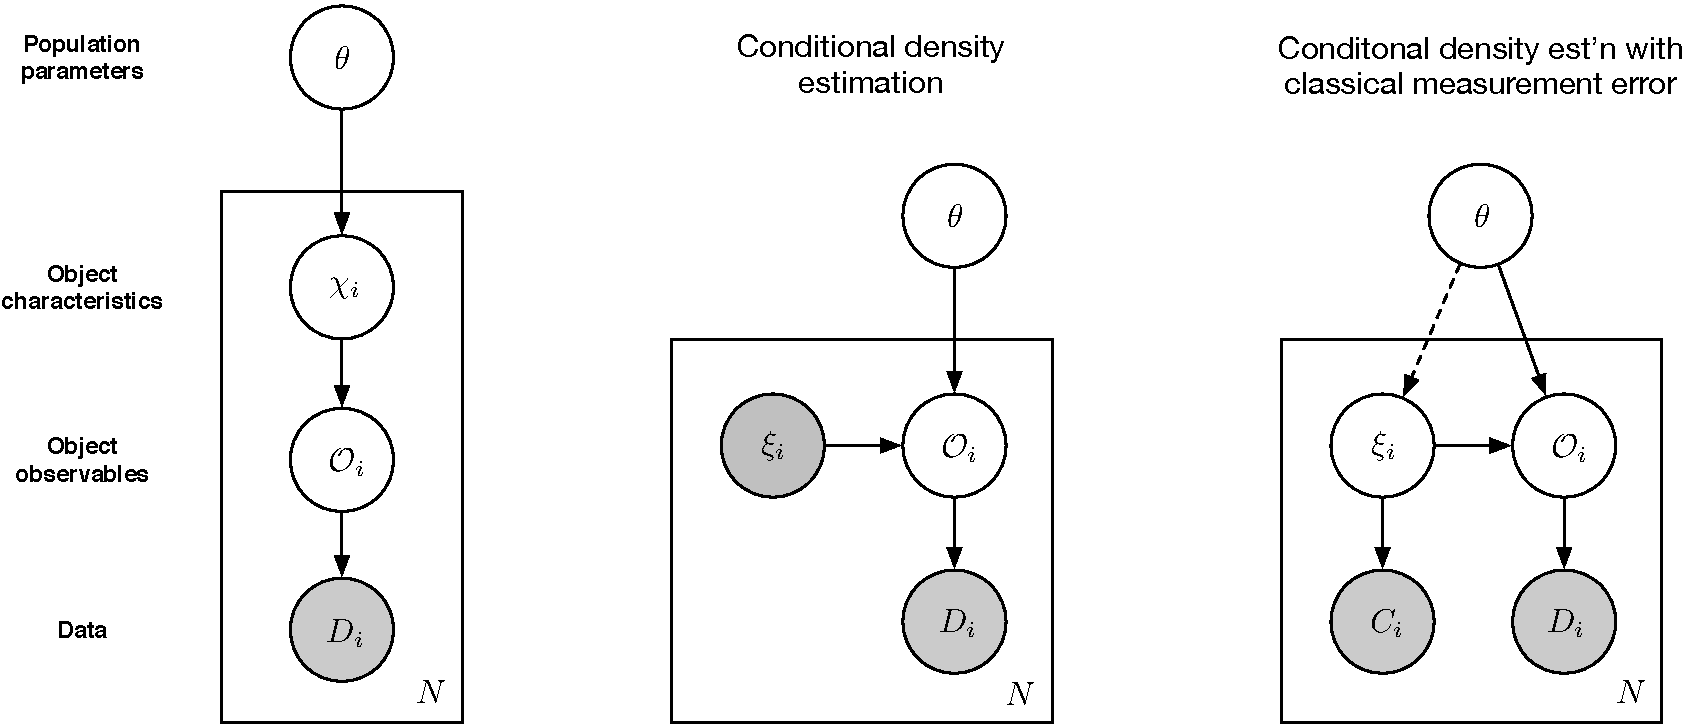
\includegraphics[width=.9\textwidth]{fig/DAGs-3}
\end{center}
\caption{Example single-plate DAGs that may be implemented in CUDAHM.
\emph{Left}: DAG for a 3-level hierarchical model corresponding to demographic inference for objects with latent characteristics $\chi_i$, related to latent observables $\obsv_i$.
\emph{Center}:~DAG for conditional density estimation, expressed via a latent observable $\obsv_i$, and a precisely measured predictor (covariate), $\xi_i$.
\emph{Right}:~DAG for conditional density estimation with classical measurement error, with a latent predictor, $\xi_i$, measured indirectly via data $C_i$.
The predictor may have an a priori known prior distribution, or it may be parameterized (with parameters included in $\theta$, in which case the dashed edge would be present).}
\label{fig:DAGs}
\end{figure}

The DAG in the left panel depicts a frequently arising structure in astronomy, where the object properties $\psi_i$ consist of intrinsic \emph{characteristics} $\chi_i$ that, if known, can predict \emph{observables}, $\obsv_i$, i.e., quantities that can predict observed data.%
\footnote{In astronomical parlance, measurements of the observables are used to ``characterize'' the object, whence our choice of the term ``characteristics'' here.
We reserve the term for properties intrinsic to the source, i.e., not depending on observer-referred quantities such as distance.
E.g., luminosity is a characteristic; flux (brightness at the telescope) is an observable.}
An important example is inference of \emph{number-size distributions} (also known as number counts or $\log N$--$\log S$ distributions).
Here the object characteristics are distance, $r_i$, and luminosity, $L_i$ (amount of energy emitted per unit time).
The observable is flux (rate of energy flow per unit area normal to the line of sight, per unit time, at the telescope), $F_i$, related to the characteristics via the inverse-square law, $F_i = L_i/(4\pi r_i^2)$ (or its cosmological generalization).

The DAG in the middle panel depicts conditional density estimation, where the properties $\psi_i$ are comprised of precisely measurable predictors (covariates), $\xi_i$, that, together with the population parameters $\theta$, specify the PDF for observables, $\obsv_i$; the data provide likelihood functions for the $\obsv_i$.
An important example is inference of a \emph{luminosity function}, which describes the population distribution for the luminosities of a class of sources (say, a stellar or galaxy type).
If the PDF for luminosity is $\lpdf(L;\theta)$, and the distances to objects may be precisely measured (say, via spectroscopic redshift data), then by a simple change of variables the PDF for the flux observable for a source at distance $d$ is $4\pi d^2 \lpdf(4\pi d^2 F; \theta)$ (in Euclidean space).
This would be the distribution for the $\obsv_i$ node in the middle DAG.
We treat a more complicated version of this problem below, where the object sample is subject to flux-dependent selection effects.

As a final example, the DAG in the right panel depicts conditional density estimation with measurement error (i.e., uncertainty in the predictors), with a classical measurement error structure (data distributions conditional on latent predictor values).
A wide variety of astronomical data analysis problems have this structure.
\cite{K+12-DustSEDs} describes a noteworthy example studying how the spectrum of infrared emission from heated interstellar dust depends on properties of the dust grains; this is one of the specific problems motivating CUDAHM.
Earlier studies, based on maximum likelihood estimates of dust properties (ignoring measurement error), found a surprising negative correlation between dust temperature and a spectral index parameter indicating how the dust properties tilt the infrared spectrum away from a black body spectrum.
Accounting for measurement error \emph{reversed the sign} of the inferred correlation, reconciling it with some theoretical models.
\cite{K+12-DustSEDs} analyzed measurements from $\sim 10^4$ dust regions; CUDAHM dramatically accelerates the calculations and makes such studies feasible with 10 to 100 times larger samples.

%-------------------------------------------------------------------------------
\subsection{CUDAHM architecture}
\label{sec:arch}

To sample member propertis in the MWG algorithm, as specified in Eq.~\ref{eq:psi_sampling}, we use the robust adaptive Metropolis (RAM) algorithm devised by \cite{vihola2012robust}.
It works by adaptively refining a Metropolis algorithm proposal distribution during the sampling process until a target mean acceptance rate $\alpha_*$ is reached.
CUDAHM currently uses a multivariate normal distribution as the proposal $q$, and sets the target mean acceptance probability to a default value of $\alpha_{*}=0.4$.
Adaptation involves using new samples to adjust the proposal covariance matrix in a manner that decays with time along the Markov chain so as to guarantee correct asymptotic sampling.
Specifically, adjustments enter with a decaying weight, $\eta_{n}=n^{-2/3}$, where $n$ is the iteration number along the Markov chain.

Following \cite{vihola2012robust}, let $S_{1}$ be the identity matrix and $X_{1}$ some point in the space to be sampled for which the target density $\pi(X_{1})>0$.
Each RAM iteration cycles through the following steps: 
\begin{enumerate} \item Compute $Y_{n}=X_{n-1}+S_{n-1}U_{n}$, where $U_{n}\sim q$ is an independent random vector.
\item With probability $\alpha_{n} \equiv \min\{1,\pi(Y_{n})/\pi(X_{n-1})\}$ the step is accepted, and $X_{n}=Y_{n}$; otherwise the step is rejected and $X_{n}=X_{n-1}$.
\item Compute the lower-diagonal matrix $S_{n}$ with positive diagonal elements satisfying the equation
\begin{equation}
S_{n}S_{n}^{T}=S_{n-1}\left(I+\eta_{n}(\alpha_{n}-\alpha_{*})\frac{U_{n}U_{n}^{T}}{\parallel U_{n}\parallel^{2}}\right)S_{n-1}^{T}
\end{equation}
where $I$ is an identity matrix.
The solution for $S_{n}$ is unique as it is the Cholesky factor of the right hand side.
\end{enumerate}
CUDAHM implements these steps on the GPU, via ``kernel'' code (code executed on a GPU) written in the CUDA language and taking advantage of optimized CUDA library functions (e.g., for random number generation and linear algebra).
The population sampling step in the MWG algorithm, as specified in Eq.~\ref{eq:theta_sampling}, is executed on the host CPU, using code written in standard \Cpp.
\enote{Are some parts of this step done on the GPU?}

%\enote{Provide some further details about the CUDAHM architecture, e.g., how users must structure their code, classes/structures available for passing information to/from the GPU, how random number generation is handled, etc..}

\enote{New text from Janos below; this needs some massaging; we also need to provide a link to the main CUDAHM repo here:}

CUDAHM enables one to easily and rapidly construct an MCMC sampler for a simple hierarchical model, requiring the user to supply only a minimimal amount of CUDA code. 
%CUDAHM assumes that a set of observed data $\{D_i\}$ are available for a sample of objects, and that these measurements are related to an unobserved set of member properties. This framework can simultaneously sample the values of these properties and the population parameters in two steps as it is mentioned earlier. The first step (2.4) is done in parallel for each object on the GPU, while the proposals for second step (2.5) are generated on the CPU, but the calculations are performed on the GPU.
There are four main classes in CUDAHM that users may need to use directly:
\begin{itemize}
\item \texttt{DataAugmentation}: This class controls the calculations involving the member properties.
\item \texttt{PopulationPar}: This class controls the calculations involving the population parameters.
\item \texttt{GibbsSampler}: This class runs the MWG sampler.
\item \texttt{GibbsSamplerWithCompactMemoryUsage}: This class also runs a MWG sampler, but with more efficient use of memory. It opens an output file stream (which has a buffer) and writes samples out on the fly.
\end{itemize}

The simplest use case involves only instantiating the \texttt{GibbsSampler} class, since this will internally construct \texttt{DataAugmentation} and \texttt{PopulationPar} objects, using reasonable default algorithms.
However, if one wants to subclass the \texttt{DataAugmentation} or \texttt{PopulationPar} classes, to customize algorithms to the problem, or to generalize the framework, then pointers to the instances of these classes must be provided to the \texttt{GibbsSampler} constructor.
In general this is only needed if one wants to override the default methods for setting the initial values, or if one wants to override the default prior on the population parameters (which is an uninformative uniform distribution).

We note the CUDAHM default methods assume \emph{all} member properties are uncertain; kernel functions that are used for updating member properties and the population parameters on the GPU assume all member properties may change in each MWG cycle.
This is important to consider for problems where the object properties contain precisely measurable predictors (e.g., covariates for conditional density estimation in the manner of the middle DAG in Fig.~\ref{fig:DAGs}), which should be held fixed over the course of posterior simulation.
When this is the case, the user should override the default methods.
The \texttt{lum\_func} implementation, which is related to the luminosity function example case, provides concrete guidance on this issue.
We are exploring internal architectural changes to simplify the user API for handling such cases.

There are two functions that the user must provide: a function that computes the logarithm of the probability density of the measurements given the member properties for each object in the sample, and a function that computes the logarithm of the probability density of the member properties given the parent population parameters.
These functions execute on the GPU and must be written in CUDA.
The file \texttt{cudahm\_blueprint.cu} under the \texttt{cudahm} directory contains a blueprint with documentation that the user may use when constructing their own MCMC sampler.
